\documentclass{article}
\usepackage[margin=1in]{geometry}
\usepackage{graphicx}
\usepackage{enumitem}
\usepackage[toc,page]{appendix}
\usepackage{amsfonts}
\usepackage{amsmath}
\usepackage{amsthm}
\usepackage{commath}
\usepackage{color}

\title{FLASH Orchestration System Design}

% No automatic indenting
\setlength\parindent{0pt}

% Set spacing between items in itemize/enumerate
\setlist{itemsep=1pt}

\newcommand{\N}                 {{\mathbb N}}
\newcommand{\Z}                 {{\mathbb Z}}
\newcommand{\Q}                 {{\mathbb Q}}
\newcommand{\R}                 {{\mathbb R}}
\newcommand{\C}                 {{\mathbb C}}
\newcommand{\F}                 {{\mathbb F}}

\newcommand{\SetuptimeParam}[1] {\textcolor{red}{#1}}
\newcommand{\RuntimeParam}[1]   {\textcolor{blue}{#1}}
\newcommand{\ComposerKey}[1]    {\textcolor{cyan}{#1}}

\newcommand{\TeamStarting}      {\textsc{TeamStarting}}
\newcommand{\TeamIdle}          {\textsc{TeamIdle}}
\newcommand{\TeamRunningOpen}   {\textsc{TeamRunningOpen}}
\newcommand{\TeamRunningClosed} {\textsc{TeamRunningClosed}}
\newcommand{\TeamRunningNoMoreWork} {\textsc{TeamRunningNoMoreWork}}
\newcommand{\TeamTerminating}   {\textsc{TeamTerminating}}

\newcommand{\ThreadStarting}    {\textsc{ThreadStarting}}
\newcommand{\ThreadIdle}        {\textsc{ThreadIdle}}
\newcommand{\ThreadComputing}   {\textsc{ThreadComputing}}
\newcommand{\ThreadWaiting}     {\textsc{ThreadWaiting}}
\newcommand{\ThreadTerminating} {\textsc{ThreadTerminating}}

\begin{document}

% Setup numbered/referentiable environment for requirements
\theoremstyle{definition} % No italics or spaces
\newtheorem{req}{Req}[section]

\maketitle

\section{Design Summary}
%The class implements a team of threads that is specifically designed for use
%by the Orchestration Runtime, which schedules a single task with the thread
%team for execution in a single cycle.  All public methods are thread-safe.
%
%The team is designed and implemented as an extended finite state machine
%(EFSM).  The mode (qualitative) portion of the EFSM's state must be in one
%and only one of
%  - Idle,
%  - Running with the work queue open
%    (i.e. able to accept more units of work),
%  - Running with the work queue closed
%    (i.e. no more units of work can be added),
%  - Running with no more pending work
%    (i.e. there are no more units of work in the queue, but at least one
%    thread is still applying the task to a unit of work), or
%  - Terminating   
%at any point in time.  The internal state variables (quantitative) for the
%EFSM are the number of
%  - pending units of work in the team's queue,
%  - Idle threads,
%  - Waiting threads,
%  - Computing threads, and 
%  - Terminating threads.
%The events that trigger state transitions are
%  - an external call to startTask()
%    (Idle -> Running \& Open),
%  - an external call to closeTask()
%    (Running \& Open -> Running Closed),
%  - a thread determines that the queue is empty
%    (Running \& Closed -> Running \& No Pending Work),
%  - all threads have transitioned to Idle
%    (Running \& No Pending Work -> Idle), and
%  - an external call results in the destruction of the thread team object
%    (Idle -> Terminating).
%At construction, the thread team starts the maximum number of threads
%allotted to it and these persist until the team is destroyed.  The EFSM
%starts in the Idle mode with all threads in the Idle state and an empty
%queue.
%
%External code starts an execution cycle by calling startTask and at the same
%time indicates what task is to be executed by the team as well as how many
%threads in the team shall be activated immediately to start applying the
%task.  After startTask has been called, external code can use the enqueue
%method to give to the team tiles on which to apply its task.  These tiles are
%passed to enqueue one unit of work at a time where a unit of work could be a
%single tile (e.g. if the task will have the team run computations on a CPU)
%or a data packet containing multiple tiles (e.g. if the task will have the
%team run computations on an accelerator).  The external code indicates to the
%EFSM that all tiles on which to operate during this cycle have already been
%enqueued.  The EFSM then continues its application of the task to all
%remaining given tiles and automatically transitions back to Idle once work
%and, therefore, the execution cycle finishes.  An external thread can be
%blocked until the task execution cycle finishes by calling the team's wait
%method.
%
%There is no restriction that a single thread team must execute the same task
%with every execution cycle.  Similarly, there is no restriction that a team
%must be dedicated to running computation-heavy code on only a single piece of
%hardware (e.g. only on the CPU or only on the GPU).  Rather, the thread team
%only knows to execute the code behind a function pointer, which can include
%kernel launches on an accelerator.  It is possible for that code to execute
%computationally-heavy code on a mixture of available HW on the node.
%However, our present best guess is that restricting each task to run
%principally on a single device is likely clean, simple, elegant, and
%maintainable.
%
%The EFSM is implemented using the State design pattern presented in the Gang
%of Four's famous Design Patterns book (Pp. 305).  This class exposes the
%interface of the EFSM to client code and the client code should only
%instantiate this class.  Each of the ThreadTeam* classes derived from
%ThreadTeamState are instantiated once by this class and are used to provide
%state-specific behavior of the team.  This design was chosen as the response
%to events, outputs, and error checking of the EFSM are logically partitioned
%across the modes of the EFSM and are therefore largely encapsulated within
%each class.  This class
%  - declares and houses all data members needed to implement the EFSM,
%  - initializes the EFSM in the correct Idle state,
%  - handles the destruction of the EFSM, and
%  - defines how all threads in the team shall behave.
%Note that each thread in the team is a FSM that moves between the Idle,
%Waiting, Computing, and Terminating states.  The hope is that studying,
%analysing, and maintaining the EFSM will hopefully be easier thanks to the
%use of this design.  However, the runtime efficiency of this design has not
%yet been studied.
%
%It is envisioned that the runtime may instantiate multiple thread teams with
%each team executing a potentially different task.  See the OrchestrationRuntime
%documentation for more information regarding this intent.
%
%To control the number of active threads running in the host at any point in
%time, a thread team can become a thread subscriber of another thread team so
%that the subscriber is notified that it can add another thread to its team
%each time a thread terminates in the publisher thread's team.
%
%To control the number of active threads running in the host at any point in
%time, a thread team can become a thread subscriber of another thread team so
%that the subscriber is notified that it can add another thread to its team
%each time a thread terminates in the publisher thread's team.
%
%In addition a thread team can also be setup as a work subscriber of another
%thread team so that when the publishing thread finishes a unit of work, the
%result is automatically enqueued on the subscriber team's queue.  When the
%publisher has finished all its work and enqueued all work units in the
%subscriber team, the publisher automatically calls the subscriber's closeTask
%method.
%
%Note that a thread publisher can only have one thread subscriber and a work
%publisher can only have one work subscriber.  However, a thread team can be
%both a thread subscriber and a thread publisher.  Also, a thread team can be
%a thread subscriber for one team and a work subscriber for another.
%
%The implementations of the publisher/subscriber design aspects are
%one-directional versions of the Observer design pattern (Pp. 293).
%
%The wait() method for a publisher team must be called before the wait()
%method of its subscriber team.

\section{Runtime Requirements}
\begin{req}
The runtime implementation and dependencies shall not impede FLASH5 from being
used on *nix operation systems including macOS nor from being run for research
on laptops.  Implementations shall not require more than the C++-11 standard and
threading implementations shall be portable.
\end{req}

\textcolor{red}{Present implementation is with pthreads, which is portable based
on OS (is it compliant with the POSIX standard).  If we do accept the C++-11
standard are reasonable, then it could be switch to use the C++ thread
facilities.}\\

\textcolor{red}{Memory managers such as AML and Umpire are dependent on
LibNuma, which is linux based.  Therefore, macOS users would presently not be
able to use a runtime based on these.  For laptops, this might be acceptable.
However, this would preclude Mac Pro users from using their GPUs.}

\begin{req}
If a simulation is setup such that no runtime is needed, then the Orchestration
runtime shall not be built into the simulation.  In particular, this means that
there shall be no unnecessary resources allocated nor an extra level of packing
tiles into data packets.  This could allow for basic stub implementations such
as initialization/finalization being called from Driver.
\end{req}

\begin{req}
At any point in time during the execution of a simulation, there shall be no more
than one instantiation of the runtime in operation so that design complexity can
be minimized (\textit{e.g.} resource allocation and management).
\end{req}

\begin{req}
The runtime shall be built into FLASH5 as a new unit and the unit shall allow
for different implementations of the unit.  Some examples of different
implementations will be
\begin{itemize}
\item{low-level (\textit{e.g.} CUDA) \textit{vs.} high-level
(\textit{e.g.} OpenMP) and}
\item{general (\textit{e.g.} CUDA) \textit{vs.}} platform-specific
(\textit{e.g.} CUDA optimized for Summit).
\end{itemize}
The interface of the runtime unit will allow for running a bundle of auxiliary
tasks and a bundle of work tasks.  \textcolor{red}{Should we allow for bundles
that are a mixture of auxiliary and work tasks?}
\end{req}

\begin{req}
The interface of the runtime shall be designed such  that when a new type of
device is introduced in platform nodes, the routines for starting a runtime
execution can be extended trivially\footnote{Ideally by adding new function
pointers to the parameter list of these routines.} for including the running of
tasks on these devices.  If the nodes allow for running concurrently tasks on
this device while running code on the host or on other devices, then the updated
interface shall allow for this.
\end{req}

\textcolor{red}{Put in information regarding runtime parameters needed by
runtime.  Does this include runtime parameters that depend upon how task were
bundled/scheduled?}\\

\textcolor{red}{Do we allow for specifying to the runtime which data should
remain where?}\\

\begin{req}
At instantiation, the runtime shall instantiate a given number, $N$, of distinct
thread teams and each thread team shall be allowed to simultaneously use
at most a given number, $M$, of threads.  \textcolor{red}{It remains to be seen
if the threads should be created at instantiation and persist throughout the
simulation or if they should be created each time the runtime executes a task
bundle.  The former would be more runtime efficient, but permanently consume
more memory in the form of thread stacks, etc. and increase the burden on the
OS.}
\end{req}

\begin{req}
Thread teams shall
\begin{enumerate}
\item{be created and run in the host CPU,}
\item{be associated with a single MPI rank,}
\item{be associated with a single unit of work (\textit{e.g.} tiles, blocks, or a
data packet of blocks), and}
\item{expose the same interface to client code regardless of the unit of work.}
\end{enumerate}
\end{req}

\begin{req}
A thread team shall execute at most one task at a time so that it is easier to
determine independence of tasks and teams.  For each task execution the client
code shall inform the thread team what task shall be executed and how many
threads in the team should be activated immediately to start work on the task.
\end{req}

\begin{req}
Thread teams shall not need to know nor be informed of which device will carry
out the computation associated with a given computational task.  Rather the
given computational task shall know where its block data resides in different
memory and the task shall be written so that it can carry out its computations
on the devices assigned to it.  This can include running code on the host CPU
with the given team thread or using the team thread to launch computations on
accelerator devices.
\end{req}

\begin{req}
Each task to be run with a thread team shall have the same identical code
interface so that task-specific information does not need to be passed to the
task by the thread team.  This requirement helps decouple the thread team and
therefore the runtime from the work being done by the runtime.
\end{req}

This implies that client code must devise a scheme that makes all
task-/computation-specific parameters available to the task function.  For
FLASH, our present design is to make all task functions methods in a unit and
all such parameters data members in the unit.  This means that the code that
calls the runtime will need to set these data members before the call.

\begin{req}
A thread team shall maintain a set of pending units of work and all threads in a
thread team shall be able to check the set of pending units of work.  In
addition, each thread in the team shall be able to claim ownership of a single
unit of work by removing it from the set with the understanding that that thread
is responsible for applying the team's task to that unit of work.  It shall be
impossible for two threads to simultaneously claim ownership of the same unit of
work.
\end{req}

\textcolor{red}{Should we allow for dividing the
load of blocks between two or more thread teams?  For example, if the task
bundle has effectively just one task, we could have half the blocks run on the
CPU and the other half on the GPU.  Should we allow for the possiblity of a
thread that determines dynamically to which thread team it should give the next
block?  This could be a way of making full use of HW.  This implies that all
thread teams in the selection pool could also be work publishers to the same
thread team that applies a follow-up task to all blocks.}

\begin{req}
A thread team shall be used by client code to apply a single, given
computational task to a subset of the blocks managed by the team's associated
MPI rank in each runtime execution cycle.  Note that the computational task can
be different with each cycle.
\end{req}

\begin{req}
The thread team interface shall allow for client code to assign units of
work to a thread team one unit at a time where the full work load given to a
team during a single task execution is a subset of the blocks managed by the
team's associated MPI rank.
\end{req}

\begin{req}
The thread team interface shall allow for client code to inform the team when
all units of work to which the current task are to be applied have been given to
the team.
\end{req}

\begin{req}
Client code shall trigger \textit{via} the runtime interface a single runtime
execution cycle that consists of executing potentially many distinct tasks on
multiple different target devices.  Based on the number of tasks in the cycle's
task bundle, the runtime will assemble the appropriate topology of thread teams.
The runtime shall trigger an error if the number of tasks in the bundle is more
than the number of thread teams created by the runtime.
\end{req}

\begin{req}
The runtime shall contain a \textbf{concurrent work distributor} that
facilitates applying multiple disctinct tasks to all the blocks managed by the
runtime's MPI rank.  Specifically, this distributor shall gather tiles using the
Grid unit's tile iterator (or asycnrhonous tile iterator), form these into the
appropriate units of work, and give the units of work to the appropriate thread
teams.  Refer to Figure~\ref{fig:ConcurrentItor} for an example of such a scheme.
\end{req}

\begin{req}
The runtime shall contain a \textbf{work splitting distributor} that facilitates
using more than one thread team in parallel to applying a single task to all the
blocks managed by the runtime's MPI rank with each the task being applied to
each block by only one team.  Specifically, this distributor shall
gather tiles using the Grid unit's tile iterator (or asycnrhonous tile
iterator), use a distribution scheme to determine which tiles will be sent to
which team, form these into the appropriate units of work based on the
destination team, and send the units of work to the appropriate thread teams.
Refer to Figure~\ref{fig:SplitItor} for an example of such a scheme.
\end{req}

\begin{req}
A thread team may be configured to push units of work, to which it has already
applied its task, to other thread teams.  The team that pushes units of work is
therefore a \textbf{work publisher} and the teams to which the units of work are
given are \textbf{work subscribers}.  A thread team shall not be allowed to push
work to itself.  It shall be possible for a single thread team to be a work
subscriber for two distinct work publishers\footnote{Split the load of blocks
between a thread team dedicated for FPGAs and a second team for GPUs.  We could
have each team run the same task on its subset of blocks and then pipe the
results into a single work subscriber that runs a quick, independent follow-up
task on the CPU.}.
\end{req}

\begin{req}
Each thread team may be configured as a \textbf{thread publisher} and as a
\textbf{thread subscriber}.  A thread publisher shall have at most one thread
subscriber and there shall be no limit to the number of thread publishers that a
thread subscriber can have.  When a thread in a thread publisher team determines
that there is no more work to be done in the current execution cycle and
therefore transitions to Idle, the thread publisher shall inform its
single\footnote{This requirement is related to load balancing and in this sense,
we cannot activate a thread in each of several thread teams because one thread
has transitioned to Idle.  We could build in a round-robin communication
scheme but choose not to in the name of simplicity.} subscriber that the
subscriber can now activate another thread in its team.
\end{req}

Note that the requirements allow for a single thread team being both a
subscriber and a publisher.

\begin{req}
A thread team shall not be allowed to push a thread or work to itself.  However,
the runtime shall not be responsible for ensuring that a given configuration of
thread teams does not lead to an endless cycle of feeding threads around a
circle of teams nor an endless cycle of feeding work around a circle of teams.
\end{req}

\begin{req}
If a thread subscriber is informed that it may activate another thread in its
team but there are no more Idle threads in the team, then the
subscriber team shall emit an error.
\end{req}

This implies that it is the client code's responsibility to ensure that the
number of threads in a thread subscriber team is less than or equal to the sum
total of threads that the team starts with and the number of threads that can be
triggered.  Note that multiple thread teams can be connected in chains and a
single thread team could be a subscriber to many chains.  Therefore, the task of
determining the maximum number of threads in a team is important.\\

\textcolor{red}{How to deal with the case of a work subscriber that has
multiple work publishers?  Publishers call a routine in subscriber to inform the
subscriber that it can detach and subscriber transitions to closed only once it
is not attached to any subscribers?  This implies pub/sub pattern with two way
knowledge of relationship.}\\

\begin{req}
The runtime shall allow for a thread team whose unit of work is a data packet of
blocks to be work publisher for a thread team whose unit of work is either a
data packet of blocks or tiles.  In the latter case, the runtime shall provide
an object that translates data packets of blocks.  For this case, this object is
the work subscriber of the first team and the work publisher of the final team.
See Figures~\ref{fig:ConcurrentItor} and~\ref{fig:SplitItor}.
\end{req}

\textcolor{red}{Is there a use case having a tile-to-data packet aggregation
object?}

\begin{req}
The runtime shall have a replay facility so that thread teams can be arranged
into a predescribed topology and each thread team setup in a given state.  This
should be useful for both debugging and designing meaningful tests.
\end{req}

\begin{figure}[!ht]
\begin{center}
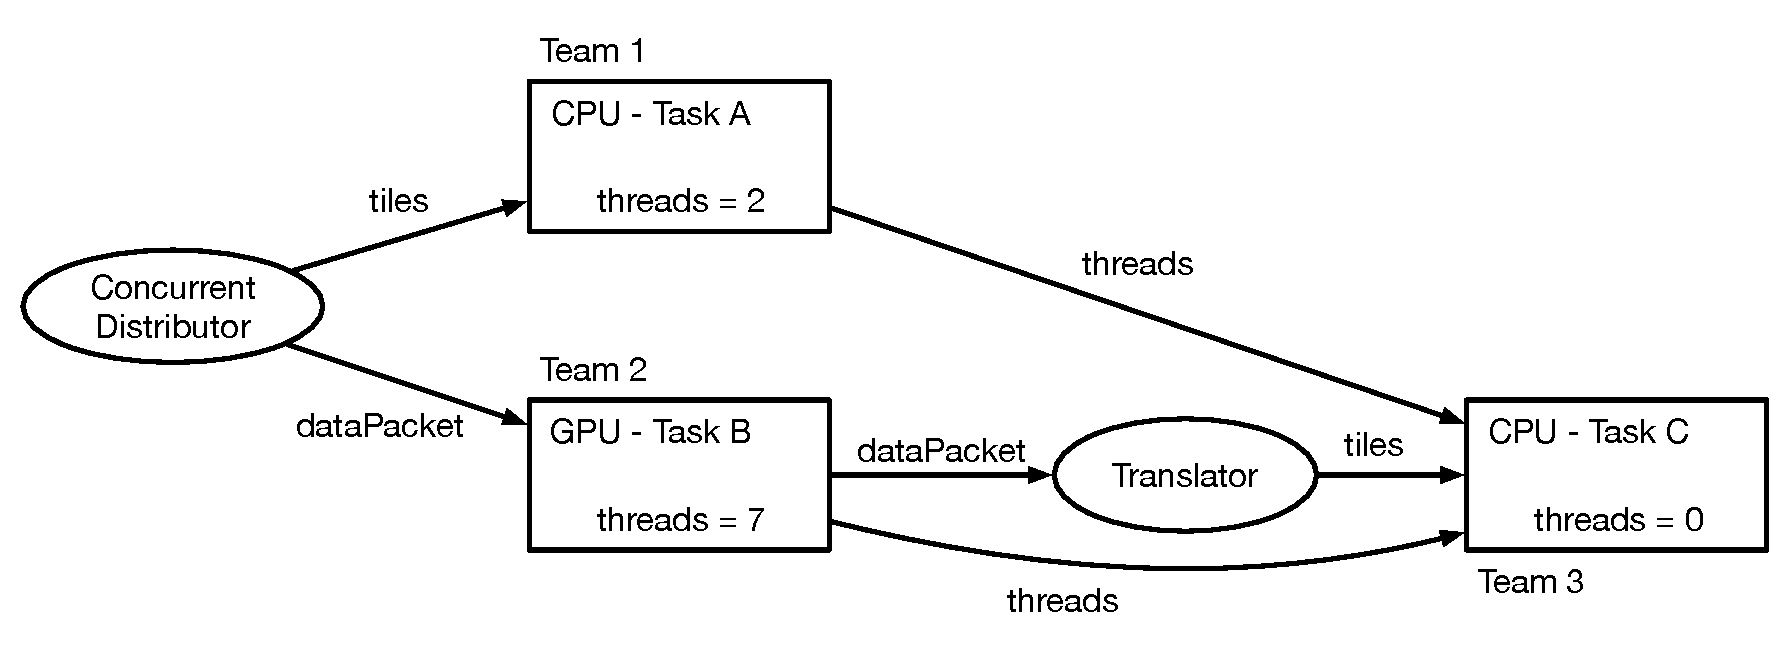
\includegraphics[width=5.0in]{ConcurrentItorExample.pdf}
\caption[]{\textcolor{red}{Add general information related to requirements.
Also specify the assumptions about RW indepence of tasks so that these
topologies will give the correct results regardless of order of execution.}}
\label{fig:ConcurrentItor}
\end{center}
\end{figure}

\begin{figure}[!ht]
\begin{center}
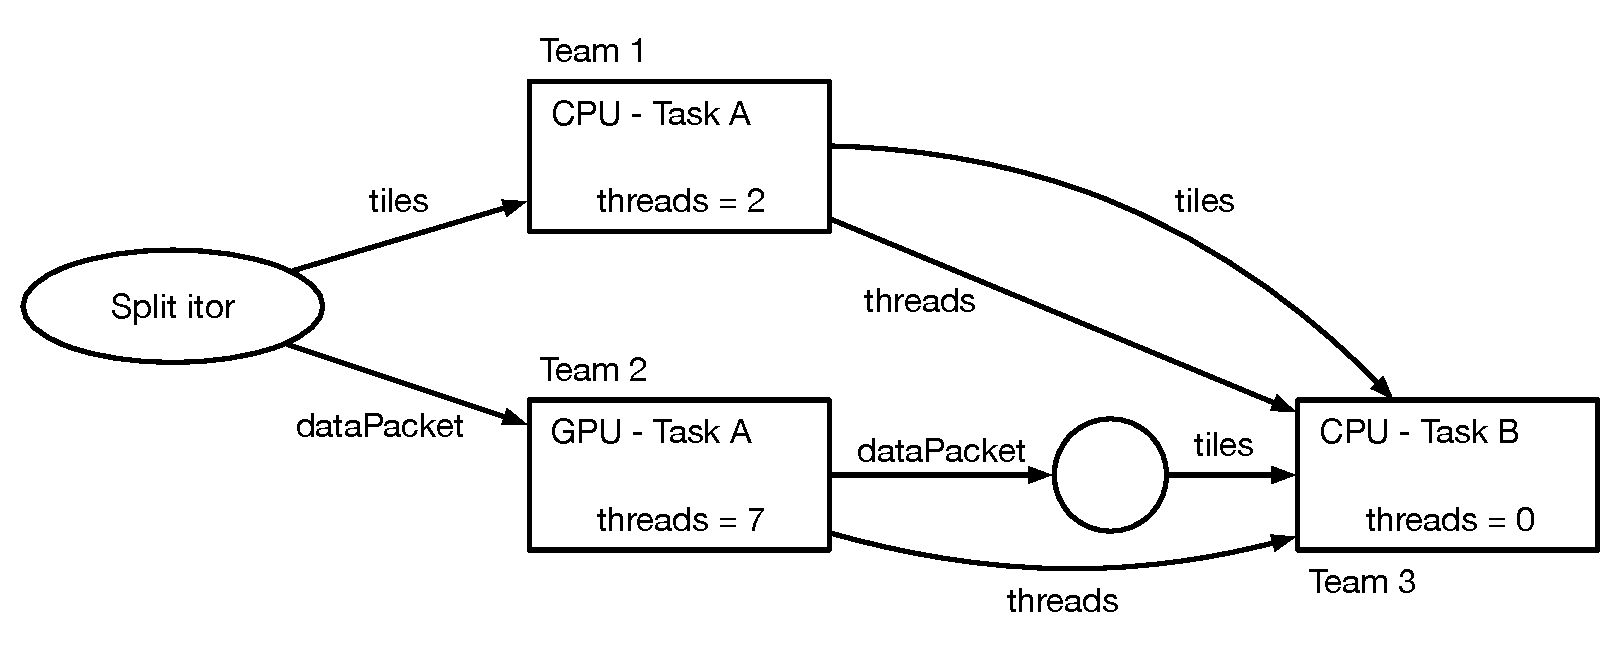
\includegraphics[width=5.0in]{WorkSplittingExample.pdf}
\caption[]{\textcolor{red}{Add general information related to requirements.
Also specify the assumptions about RW indepence of tasks so that these
topologies will give the correct results regardless of order of execution.}}
\label{fig:SplitItor}
\end{center}
\end{figure}

\section{Runtime Technical Specifications \& Design}
%What classes of scalar values do we have in the physics units?  For instance are
%there scalars that are constant for the duration of the simulation?  Constant
%for the duration of an iteration?  Constants that are changed by auxiliary
%tasks?  Constants that are updated by work tasks?  For the first two, we can set
%up mirrors of the variable between host and devices.  Those that are changed by
%auxiliary tasks can also be mirrored by running the task concurrently in both
%the CPU and the GPU.  What about the others?  Do we send those in the data
%packets so that the CPU and GPUs can force the mirroring somehow?  Do we just
%hand these over the managed memory and hope that everything goes well?  Do we
%hand these over to managed memory but ask the task composer to touch the scalars
%on the appropriate device before each runtime call (these are blocking)?\\

\subsection{Thread Teams}
A thread team is fundamentally event-driven software and as such its design
has been specified as a finite state machine.  However, the behavior in a given
state cannot be specified solely on the basis of a single qualitative state
variable.  Rather, the behavior will depend on a qualitative state variable,
which is called the mode, as well as the quantitative internal state variables
$N_i, N_w, N_c, N_Q$ that respectively keep track of 
\begin{itemize}
\item{the number of idle threads in the team,}
\item{the number of threads that are waiting for work to be added,}
\item{the number of threads executing a computation on a unit of work, and}
\item{the number of units of work in the team's pending work queue.}
\end{itemize}
Note that the definitions of $N_i, N_w, N_c$ imply that each thread is
always in one and only one state but that this EFSM need not track the actual
state of each thread --- it is only the aggregated thread state information that
is important.  Therefore, the runtime is an extended finite state machine 
\[
M = (Q, X, I, O, s_0, T)
\]
where
\begin{itemize}
\item{$Q$ is the finite set of qualitative modes,}
\item{$X = \set{(N_i, N_w, N_c, N_Q) \in \Z_{\ge 0}^4\,|\,N_i + N_w + N_c =
N_{max}}$ is the set of internal state variables where $N_{max}$ is the
number of threads in the team,}
\item{$I$ is the set of internel and external events,}
\item{$O$ is the set of outputs,}
\item{$s_0 = (q_0, x_0) \in Q \times X$ is the initial state, and}
\item{$T : Q \times X \times I \to Q \times X \times O$ is the transition
function that is evaluated by the EFSM at each occurrence of an event to
identify the output to be performed as well as the state to transition to.}
\end{itemize}

The set $Q$ contains the modes
\begin{itemize}
\item{\TeamIdle --- all threads idle and no work in the queue}
\item{\TeamRunningOpen --- a task has been given to the team and units of work
on which to execute the task can still be given to the team}
\item{\TeamRunningClosed --- a task being executed but no more units
of work can be given to the team}
\item{\TeamRunningNoMoreWork --- a task is being executed, no more
units of work can be given, and the team has identified that the task has
already been applied to or is currently being applied to all units of work}
%\item{\TeamTerminating --- the client has indicated that it no longer needs the team.}
\end{itemize}

The set $I$ of events is the union of events triggered by clients through the
team's interface
\begin{itemize}
\item{\texttt{startTask} --- give the team a task and activate a given number of the
$N_{max}$ idle threads in the team to work on it}
\item{\texttt{increaseThreadCount} --- activate a given number of idle threads in the
team so that they can start working on the task as well}
\item{\texttt{enqueue} --- give the team a unit of work on which to apply its
task}
\item{\texttt{closeTask} --- indicate (without blocking the caller) to the team
that no more units of work will be given for the current task}
%\item{\texttt{$\sim$ThreadTeam} --- thread team no longer needed}
\end{itemize}
with the set of events triggered internally
\begin{itemize}
\item{\texttt{activateThread} --- wake an idle thread so that it can participate
in applying a task to given units of work}
\item{\texttt{transitionThread} --- wake a thread that is waiting for work so
that it can evaluate if there is pending work and update its state accordingly}
\item{\texttt{computationFinished} --- a thread finished applying the team's
task to a unit of work and shall evaluate if there is pending work and update
its state accordingly}
%\item{\texttt{threadTerminated} --- emitted by a thread to indicate that it has
%terminated}
\end{itemize}

\textcolor{red}{Add in explanation of how computationFinished is different and
how it could be perceived to break the rules of a FSM since the thread never
finishes its transitions.  With the right definitions, it seems that we get
around this --- the thread is is an effective blocking state (i.e. like waiting
of a signal) while it is computing.  This signal is only emitted by a computing
thread and is only received by the emitting thread itself.}

The initial state is defined to be
\[
s_0 = \left(q_0, (N_i, N_w, N_c, N_Q)_0\right) = \left(\TeamIdle, (0, 0, 0, 0)\right).
\]

The set $O$ and the transition function $T$ encapsulate the complexity of the
runtime and are specified in the spreadsheet XXX.  A state diagram for the team
that indicates only states and transitions is shown in
Figure~\ref{fig:TeamStateDiagram}.  A similar state diagram for threads in the
team is shown in Figure~\ref{fig:ThreadStateDiagram}.  These figures are
intended only to aid in understanding the design of the runtime.  The content of
XXX should be understood to be the actual design of the runtime.\\

The design and implementation philosophy of the EFSM was to put an emphasize on
correctness and maintainability.  One important consequence was to create a
design that accounts for all possible states/transitions/events even though it
could be proven that some states/transitions/events are precluded from happening
by the design itself.  Therefore, our design/implementation is hopefully robust
and not so sensitive to small design changes.  Also, the mental load associated
with working with the design is lower since we do not have the burden of proving
and maintaining proofs of impossible states/transitions.  This is especially
important as the thread-based implementation of the thread team cannot make
strong assumptions about the predictability of the order of execution of code
and events, which increases the complexity of such proofs.  This is ugly in the
sense that the code might carry out actions that it shouldn't without our
knowing.  It always means that we have not completely understood the full
behavior of the EFSM.

\begin{figure}[!ht]
\begin{center}
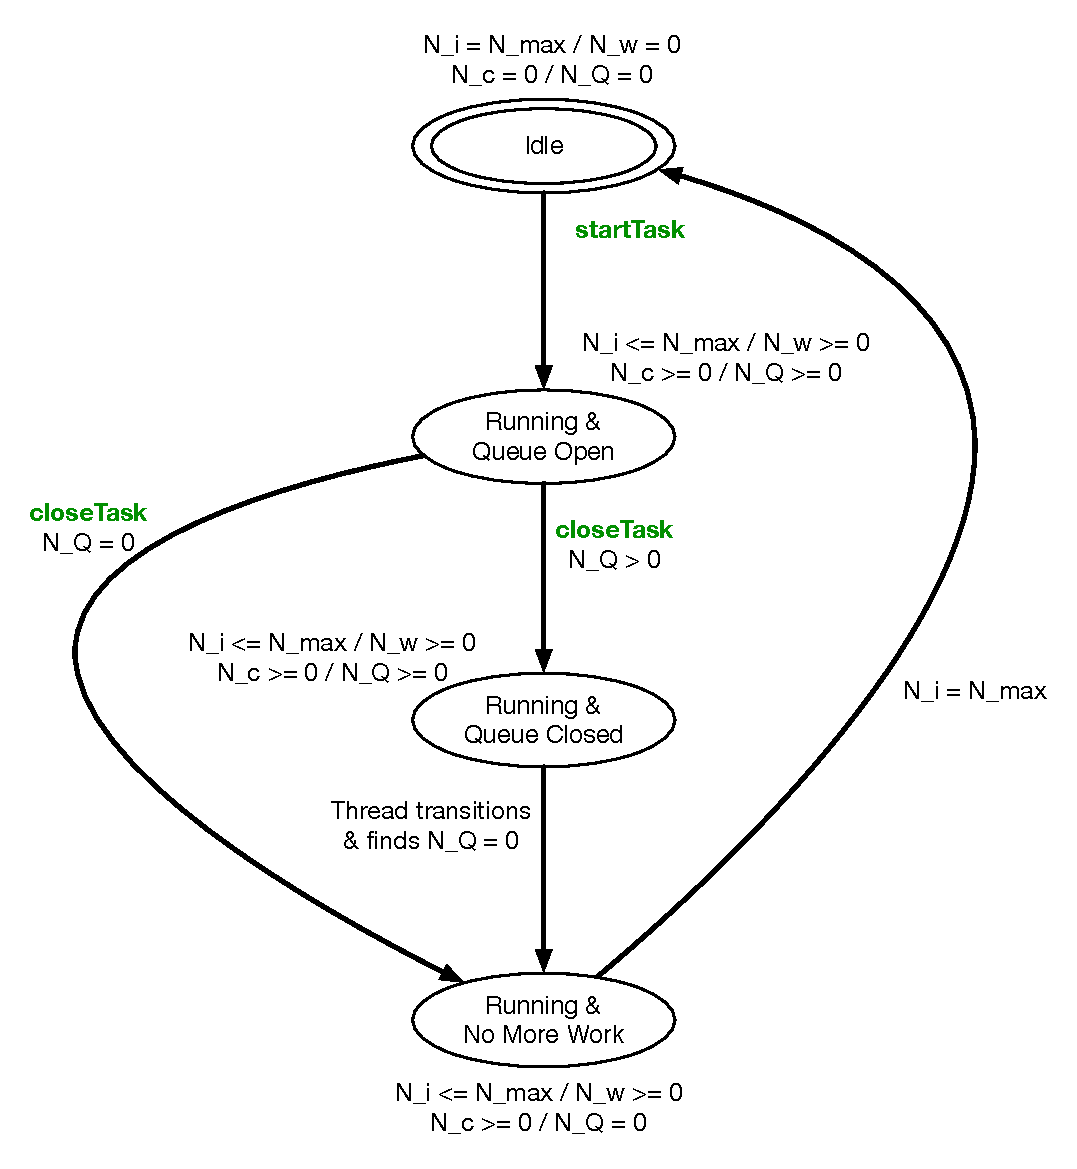
\includegraphics[width=5.0in]{TeamStates.pdf}
\caption[]{}
\label{fig:TeamStateDiagram}
\end{center}
\end{figure}

\begin{figure}[!hp]
\begin{center}
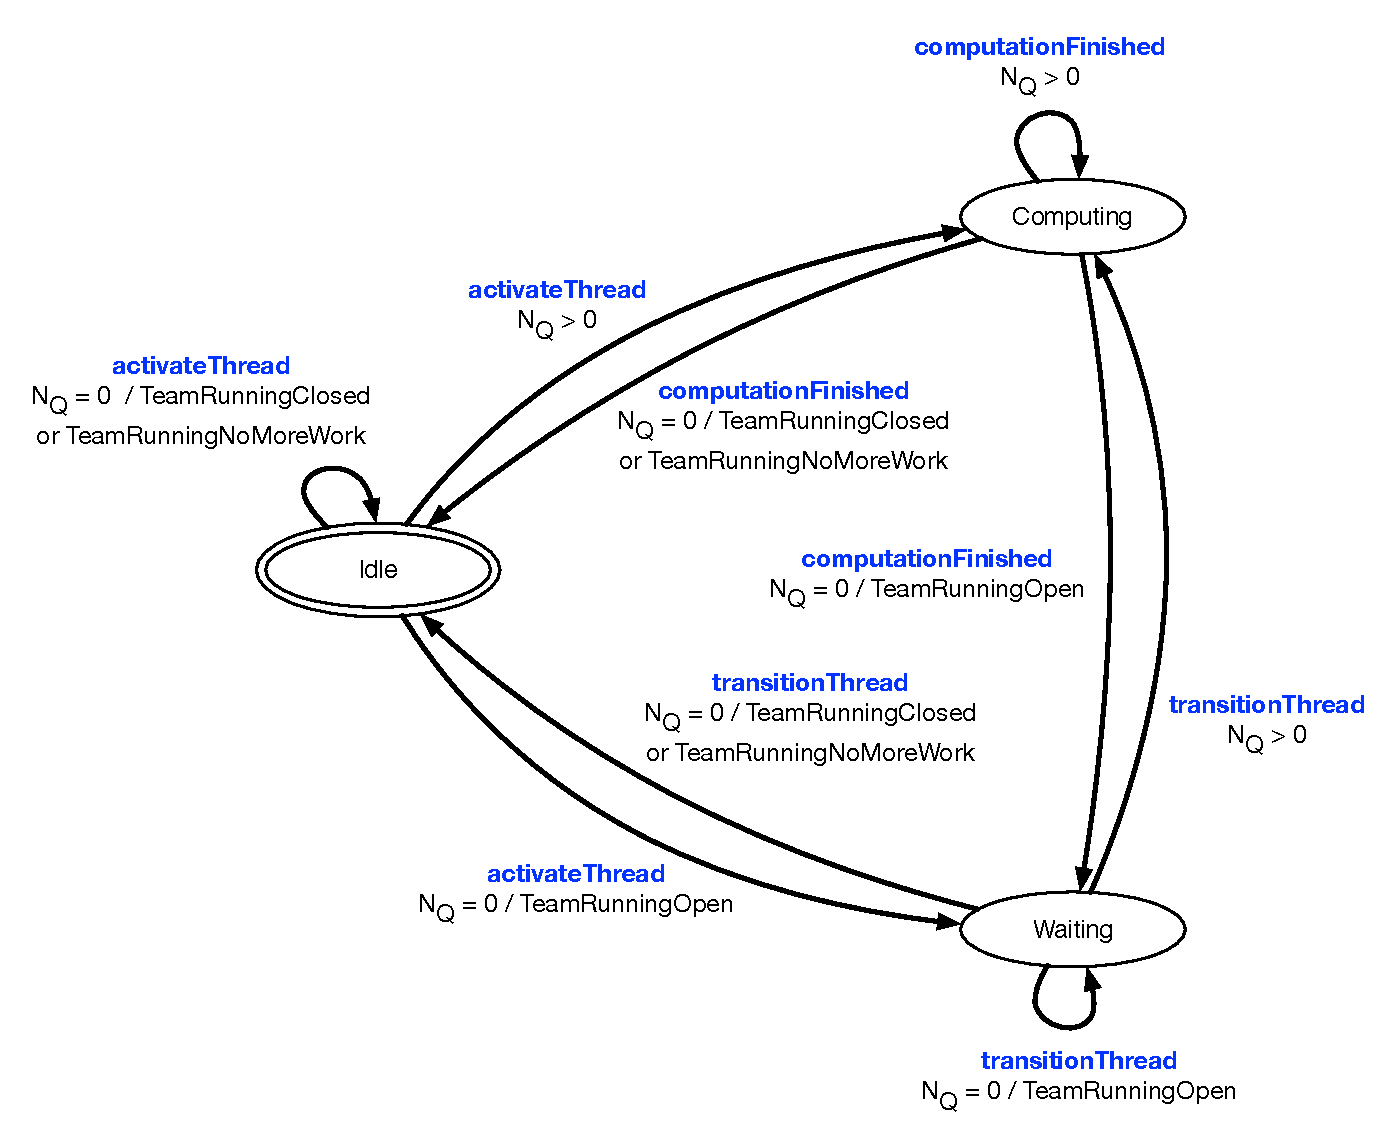
\includegraphics[width=6.5in]{ThreadStatesPersistent.pdf}
\caption[]{}
\label{fig:ThreadStateDiagram}
\end{center}
\end{figure}

\begin{req}
All threads that transition to idle must wait for the \texttt{activateThread}
signal.
\label{req:IdleActivateThread}
\end{req}

\begin{req}
External code can decrease $N_i$ through the \texttt{startTask} and
\texttt{increaseThreadCount} events and the runtime shall be implemented such
that a request to activate $i$ threads results in an error if $i$ exceeds the
number of idle threads that are available for activation.
\end{req}
\textbf{Verification:}\hspace{0.125in}  In the present design, this requirement
is important because the runtime would emit more \texttt{activateThread} signals
than there are threads to receive them.  Because teams allows for thread
publishers/subscribers, undetected signals would amount to a loss of thread
resources at the level of the runtime.  Note that a thread-based implementation
will have a lag between when these events trigger the activation of idle threads
and when these threads are actually activated.  The runtime design therefore
tracks the actual number of idle threads with \texttt{N\_idle\_} = $N_i$ as well
as the number of threads pending activation with \texttt{N\_to\_activate\_}.
When a thread does receive \texttt{activateThread}, it decrements both
\texttt{N\_idle\_} and \texttt{N\_to\_activate\_} and increments the internal
state variable $N_i, N_w$ or $N_c$ corresponding to the thread's next state.
To satisfy the requirement, both events throw an error if $i > $
\texttt{N\_idle\_} - \texttt{N\_to\_activate\_}.

\begin{req}
\label{req:Runtime_OneWait}
The interface of the thread team shall contain a \texttt{wait} method so that
for each task execution, the execution of a thread that calls \texttt{wait} is
blocked until the termination of the task.  This interface shall allow for at
most one thread to block its execution with this method during each task
execution.
\end{req}
\textbf{Verification:}\hspace{0.125in}  Implemented a flag
\texttt{isWaitBlocking\_} to track if a thread has already called \texttt{wait}.

\textcolor{red}{Should we have a variant of wait that accepts a timeout?}

\begin{req}
To maintain a simple design, client code shall only be allowed to attach and
detach thread subscribers when the team is in the {\TeamIdle} mode.  The same
requirement applies for work subscribers.
\end{req}
\textbf{Verification:}\hspace{0.125in} Implemented directly as stated.

\begin{req}
In the original designs, the Team state machine also contained a
{\TeamTerminating} mode.  The transition to this mode was allowed only from
{\TeamIdle} and was triggered by initiating the destruction of the team.  While
sensible, this design was flawed since a runtime error that occurs with the team
in any state could trigger the destruction of the team.  Therefore, the
termination of the EFSM and the clean-up of its resources shall be possible from
any state.
\end{req}
\textbf{Verification:}\hspace{0.125in}  The destructor does not do any error
checking to confirm that destruction was called with the EFSM in any particular
state.  Also, the destructor assumes that there are Idle, Waiting, and Computing
threads at the time of calling.  For the Idle and Waiting threads, it triggers
them to finish; the Computing, it waits for them to finish their work and
discover that they should terminate.

\begin{req}
\label{req:Runtime_AtomicTransition}
As per the requirements of FSMs, each transition shall be implemented so that
the code executing the transition has sole access to the thread team's state
during the entirety of the transition.  This implies that no other thread can
alter the state simultaneously.
\end{req}
\textbf{Verification:}\hspace{0.125in}  With each change to the software, the
satisfication of this requirement should be reverified.\\

Given the present implementation, it important for transitions that transition
the mode and emit internal signals that the code transition the mode
\textbf{first} and then emit the signals.  This is to prevent the possible
(\textbf{TBC} for pthreads?) case that the signal is emitted and received
before the mode is correctly transitioned, which would violate
Requirement~\ref{req:Runtime_AtomicTransition} and cause the responding thread
to react to the signal is a way that is potentially not in accord with the true
mode of the EFSM.

\begin{req}
Any transition to {\TeamRunningNoMoreWork} shall awaken all waiting threads so
that they can transition to Idle.
\end{req}
\textbf{Verification:}\hspace{0.125in}  Implemented directly as stated.

\begin{req}
Any transition to {\TeamIdle} shall call the \texttt{closeTask()} method of the
team's work subscriber if it has a work subscriber.
\end{req}
\textbf{Verification:}\hspace{0.125in}  Implemented directly as stated.

\begin{req}
Upon emitting/receiving the \texttt{computationFinished} signal, a computing
thread shall enqueue the unit of work that it just finished applying the team's
task to with the team's work subscriber if the team has a work subscriber.
\end{req}
\textbf{Verification:}\hspace{0.125in}  Implemented directly as stated.

\begin{req}
\end{req}
\textbf{Verification:}\hspace{0.125in}

\subsection{{\TeamIdle} State}
\begin{req}
\label{req:Idle_NoEnqueue}
While the runtime could allow clients to give units of work to a team with the
understanding that the work would be for the next task to be given to the team,
there is no known use case for which this is necessary.  Therefore, to simplify
the design, client code shall not be allowed to give a team a unit of work if
the team is in the mode \TeamIdle.  
\end{req}
\textbf{Verification:}\hspace{0.125in}  The \texttt{enqueue} method throws an
error if called in this mode.  There is no other means to add work.\\

Given this requirement, it would be wise to call \texttt{startTask} on all
thread teams to be used on a task before enqueueing work with any of these.  This
practice will help avoid the case where an active work publisher tries to
enqueue work on a work subscriber that is still in the mode \TeamIdle.

\begin{req}
In the {\TeamIdle} mode, the queue shall always be empty and all threads in the
team in the idle state.  This implies that no thread can be in the Waiting,
Computing, or Terminating states and that all threads are therefore by
Req~\ref{req:IdleActivateThread} are waiting to receive the
\texttt{activateThread} event.
\end{req}
\textbf{Verification:}\hspace{0.125in}  The initial state starts in {\TeamIdle}
but specifies that there is no work in the queue.  Also, all transitions to
{\TeamIdle} can only happen if the queue is empty.  Therefore, the pending work
queue is always empty upon entry to \TeamIdle.  Finally, no work can be added
to the queue in the {\TeamIdle} state by Req~\ref{req:Idle_NoEnqueue}.\\

The initial state specifies that all threads are idle and transitions to
{\TeamIdle} can only happen if the same is true.  Therefore, the claim is true
upon entry to {\TeamIdle} and all threads are waiting for \texttt{activateThread}.
Also, responses\footnote{These cases are being considered should one of these
events be emitted when the team in not Idle, but is received after transitioning
to Idle.  With the current implementation, since all threads would be waiting on
\texttt{activateThread}, no threads would be waiting for the latter two events.}
to \texttt{activateThread}, \texttt{transitionThread}, and
\texttt{computationFinishes} do not transition the thread state and have the
responding threads wait for \texttt{activateThread}.  Therefore any attempt to
transition a thread terminates with the thread in idle.

\begin{req}
Consider a team that is both a thread publisher and subscriber.  It is possible
for the team to finish its work and transition to {\TeamIdle} before its
publisher finishes its work.  Therefore, to avoid loss of thread resources at
the level of the runtime, teams that are thread publishers and that are in
{\TeamIdle} shall forward requests to increase thread count on to their
subscriber.
\end{req}
\textbf{Verification:}\hspace{0.125in}  Implemented directly as stated.

\begin{req}
It is possible that a runtime execution cycle could finish and transition the
team back to {\TeamIdle} before an external thread has the chance to call
\texttt{wait}.  Therefore, the method shall be enabled in {\TeamIdle} and shall
terminate immediately to avoid unnecessary blocking of the calling thread.  Note
that this does allow for client code to superfluously call \texttt{wait} before
the first execution cycle is run and multiple times between cycles, both of
which are logical errors.
\end{req}
\textbf{Verification:}\hspace{0.125in}  Implemented directly as stated and in
accord with Req~\ref{req:Runtime_OneWait}.  

\subsection{\TeamRunningOpen}
\begin{req}
Consider the case of two teams, one of which is the work publisher for the
other.  When the publisher team transitions to {\TeamRunningNoMoreWork}, it
calls the subscriber's \texttt{closeTask()} method to inform the subscriber that
it will not be given more work.  This implies that the thread that executes an
execution cycle with the Orchestration Runtime does not know when
\texttt{closeTask()} is called and therefore could call \texttt{wait()} before
this event occurs.  Hence, a thread team in the state {\TeamRunningOpen} shall
allow for a thread to call \texttt{wait()} method.
\end{req}
\textbf{Verification:}\hspace{0.125in}  Implemented directly as stated.

\begin{req}
\end{req}
\textbf{Verification:}\hspace{0.125in}

\subsection{Possible Requirements}
%If a thread team is going to ship data to an accelerator like a GPU, then the
%unit of work for such a thread team shall be a data packet of tiles (with the
%possibility that the tiles are the trivial tiling).  This includes the
%possibility of data packets that consist of a single tile (and therefore tile
%that consist of a single block). 

%If a thread team is going to ship data to the host, then the unit of work for
%such a thread team shall be a tile (with the possibility that the tiles are the
%trivial tiling).

The queue thread shall create the iterator indicated to it by the parameters
passed to executeTask and shall be able to form all necessary units of work from
this.  This is too specific.  What if it can just queue tiles to every team and
the units of work are formed at dequeueing?  Who is responsible for the
shipments then?  Who is responsible for bringing data back?

%If thread team A and thread team B have different units of work and team B is a
%work subscriber of A, then there shall exist a mechanism in the
%enqueueing/dequeueing process for translating units of work.
%\textcolor{red}{This is not yet resolved.  For example, we could ask the
%publishers to do the translation --- enqueue each tile in a data packet
%separately or assemble tiles into data packets.  Or, when a task execution cycle
%is initiated, each subscriber team would create a queue that receives the work
%unit of its publisher and dequeueing would do the translation.}.  Can we relax
%this so that data packets are only assembled by the queue task and all GPU-based
%teams that receive work from a CPU-based team have single tile data packets?
%Can our pipeline eventually hide the explosion of transport latency costs?  This
%seems unlikely since tile size is set for the CPU and could lead to units of
%work too small to keep the GPU busy for long enough to hide the latencies.

%Should we allow the Post-concurrency task to start immediately when blocks get
%back from the GPU?  This would imply that this task is also independent from the
%CPU-concurrent task.  Or, do we run the Post-concurrent task only after both the
%CPU and GPU work have finished?  Note that we can never know that a single
%routine will always run on either the host or either the device.  They must be
%written in such a way that they can be run well on either without manual or
%automatically updating the code beyond directives (OpenACC, OpenMP, CUDA, etc.).\\

%Consider a unit of runtime work that includes a GPU-concurrent task, a
%CPU-concurrent task, and a Post-concurrency CPU task in its task bundle.  Then
%for each block in a data packet, the concurrent CPU task will have blocks of
%input data (CC, FC[XYZ], Fluxes[XYZ], etc.), output data (CC, FC[XYZ],
%Fluxes[XYZ], etc.), and scratch blocks (e.g. grav[XYZ], auxC).  The concurrent
%GPU task will have the same, but non-intersecting block structure.  The
%post-concurrency CPU task can use whatever is in MFabs that is not being worked
%on by the concurrent CPU task and can allocate its own CPU scratch blocks.  We
%can get the CPU scratch memory through the runtime memory manager, but I don't
%know if we need to manage that memory or just let failures happen.  This assumes
%that the host memory will never be the limiting memory pool factor (i.e. that
%the host memory will always be much larger than the device memory).\\

%It is possible that certain units of runtime work will not need to bring the
%data back to the host memory as that same data is needed by the next runtime
%execution in the same device.  However, since we cannot assume that all the
%memory will fit in the device memory, we must assume that in the worst case only
%a fraction of the intended blocks will stay in the device memory.  The runtime
%shall maintain location information for each block that persists across calls to
%the runtime.  When the next runtime execution begins, those blocks already in
%the device shall be grouped into one or more data packets and work immediately
%launched on these.  The runtime shall not include these same blocks in a
%subsequent data packet so that we avoid repeated work.  FLASH shall abort
%execution if, at the end of a time step, we have blocks of persistent data
%(\textit{e.g.} unk) that are not in the host memory.  \textcolor{red}{Are these
%really requirements that we want?  If yes, then the blocks in the device memory
%would be the first data packet and therefore we get the pipeline up and running
%quicker.}  Example of this is unsplit Hydro.  The computeFluxes routine pulls in
%the UNK data on CC1 and updates the fluxes.  Neither needs to go back to the GPU
%ever.  The updated solution is in CC2.  Note that if we have the future case of
%host and some devices sharing the same physical memory, this requirement could
%become more imporatant.  Therefore, giving the runtime more parameters to inform
%data movements could be important.\\

%\newpage
%\begin{appendices}
%\section{Hydro operations}
%The Unsplit implementation of the Hydro step operation has at least three
%variants and the variant executed at runtime is presently determined at each
%time step based on the Grid unit AMR implementation chosen (known at setup) 
%and whether or not flux correction should be applied (specified as a runtime
%parameter).  Here we express each variant as an operation.\\
%
%\textcolor{red}{TODO: Add to requirements that parameter such as flux correction
%should be both a setup and runtime parameter.  If the setup-time value is false,
%then the task scheduler has the possibility to fuse tasks.  If it is true, then
%the runtime parameter can still be set to turn this off.  However, the binary
%built will not have been built with the potential for fusing tasks.}\\
%
%For the following subsections, the colorization is
%\begin{itemize}
%\item{a \ComposerKey{keyword} that is paired with a static Fortran routine in
%the operation's dictionary,}
%\item{a \RuntimeParam{runtime} parameter, and}
%\item{a \SetuptimeParam{setup-time} and runtime parameter.}
%\end{itemize}
%
%TODO: Add in a UG variant?!
%
%\newpage
%\subsection{No flux correction variant}
%\texttt{
%\begin{tabbing}
%\hspace*{0.25in}\=\hspace*{0.25in}\= \kill
%if \SetuptimeParam{shockDetectOn}:\\
%\>\ComposerKey{GcFillWithoutEoS} (global, internode data movement)\\
%\> Task 1:\\
%\>\> \ComposerKey{doShockDetection}\\
%\ComposerKey{GcFillWithEoS} (global, internode data movement)\\
%Task 2:\\
%\> if \RuntimeParam{updateHydroFluxes}:\\
%\>\> \ComposerKey{updateHydroData}\\
%\> \ComposerKey{zeroFluxData}\\
%\> iterate \ComposerKey{LeavesWithoutTiling}:\\
%\>\> \ComposerKey{computeFluxesAndUpdateSolution}\\
%\end{tabbing}
%}
%
%For \ComposerKey{computeFluxesAndUpdateSolution}, the dictionary should know
%that it needs to run \texttt{hy\_computeFluxes} with \texttt{Uout => Uin}.
%
%\subsection{Paramesh + flux correction variant}
%\texttt{
%\begin{tabbing}
%\hspace*{0.25in}\=\hspace*{0.25in}\=\hspace*{0.25in}\= \kill
%if \SetuptimeParam{shockDetectOn}:\\
%\>\ComposerKey{GcFillWithoutEoS} (global, internode data movement)\\
%\> Task 1:\\
%\>\> \ComposerKey{doShockDetection}\\
%\ComposerKey{GcFillWithEoS} (global, internode data movement)\\
%Task 2:\\
%\> if \RuntimeParam{updateHydroFluxes}:\\
%\>\> \ComposerKey{updateHydroData}\\
%\> \ComposerKey{zeroFluxData}\\
%\> iterate \ComposerKey{LeavesWithoutTiling}:\\
%\>\> if level == finest:\\
%\>\>\> \ComposerKey{computeFluxesAndUpdateSolution}\\
%\>\> else:\\
%\>\>\> \ComposerKey{computeFluxes}\\
%\> \ComposerKey{storeFluxDataForFluxCorrect}\\
%\ComposerKey{conserveFluxes} (global, internode data movement)\\
%Task 3:\\
%\> iterate \ComposerKey{LeavesWithoutTiling}:\\
%\>\> if level == finest:\\
%\>\>\> \ComposerKey{noOp}\\
%\>\> else:\\
%\>\>\> \ComposerKey{updateSolution}\\
%\> \ComposerKey{updateBoundaries}
%\end{tabbing}
%}
%
%\newpage
%\subsection{AMReX + flux correction variant - tiling}  
%\textbf{Input:} \texttt{simTime, dt, dtOld, sweepOrder}\\
%\textbf{Output:} the updated solution with EoS run on all leaf blocks.  GC data
%not necessarily good.
%
%\texttt{
%\begin{tabbing}
%\hspace*{0.25in}\=\hspace*{0.25in}\=\hspace*{0.25in}\=\hspace*{0.25in}\= \kill
%if \SetuptimeParam{shockDetectOn}:\\
%\>\ComposerKey{GcFillWithoutEoS} (global, internode data movement)\\
%\> Task 1:\\
%\>\> iterate \ComposerKey{LeavesOnLevelWithoutTiling}:\\
%\>\>\> \ComposerKey{doShockDetection} (operates on single block)\\
%\ComposerKey{GcFillWithEoS} (global, internode data movement)\\
%Task 2:\\
%\> if \RuntimeParam{updateHydroFluxes}:\\
%\>\> SubTask 2.1 (Run in device so that data is already in device memory?):\\
%\>\>\> \ComposerKey{updateHydroData} (doesn't operate on blocks, but sets
%variables)\\
%\> SubTask 2.2 (Run in CPU to avoid data movements?):\\
%\>\> \ComposerKey{zeroFluxData} (iterates over all leaf blocks)\\
%\ComposerKey{TaskBarrier} (fake data movement so that tasks are clean and efficient)\\
%Task 3:\\
%\> level = finest\\
%\> iterate \ComposerKey{LeavesOnLevelWithoutTiling}:\\
%\>\> \ComposerKey{computeFluxesAndUpdateSolution}\\
%\> if \ComposerKey{nLevels} > 1:\\
%\>\> \ComposerKey{storeFluxDataForFluxCorrect}\\
%\> level = finest-1 (NOTE: There might only be one level at any iteration!)\\
%\> iterate \ComposerKey{LeavesOnLevelWithoutTiling}:\\
%\>\> \ComposerKey{computeFluxes}\\
%\> if level != coarsest:\\
%\>\> \ComposerKey{storeFluxDataForFluxCorrect}\\
%\ComposerKey{conserveFluxes} (global, internode data movement)\\
%loop level=finest-1..coarsest:\\
%\>Task 3+i:\\
%\>\> iterate \ComposerKey{LeavesOnLevelWithoutTiling}:\\
%\>\>\> \ComposerKey{updateSolution}\\
%\>\> level = finest-i\\
%\>\> iterate \ComposerKey{LeavesOnLevelWithoutTiling}:\\
%\>\>\> \ComposerKey{computeFluxes}\\
%\>\> if level != coarsest:\\
%\>\>\> \ComposerKey{storeFluxDataForFluxCorrect}\\
%\ComposerKey{conserveFluxes} (global, internode data movement)\\[0.25in]
%Task M:\\
%if \SetuptimeParam{useGravity}:\\
%\> \ComposerKey{prepareNewGravityAccelerations}\\
%\ComposerKey{doGravityStep}
%\ComposerKey{TaskBarrier} (Implied because we are at the end of the operation?)
%\end{tabbing}
%}
%
%Note that \texttt{hy\_updateSolution} calls \texttt{hy\_energyFix} and \texttt{Eos\_wrapped}
%at the end.  These two could be pulled out and included as subtasks that could
%be run on the CPU after \texttt{hy\_updateSolution} finishes running on a data
%packet in the accelerator.\\
%
%Note that \texttt{hy\_prepareNewGravityAccelerations} can call
%Gravity\_potential and GcFill in the end.  This needs to be moved up.\\
%
%Note that \texttt{hy\_gravityStep} iterates over all leaf blocks to update the
%solution using the gravity accelerations.
%
%\end{appendices}

\end{document}
